
  \subsubsection{Front-end}
  \paragraph{Informazioni sul package}
    \begin{figure}[H] 
      \begin{center} 
        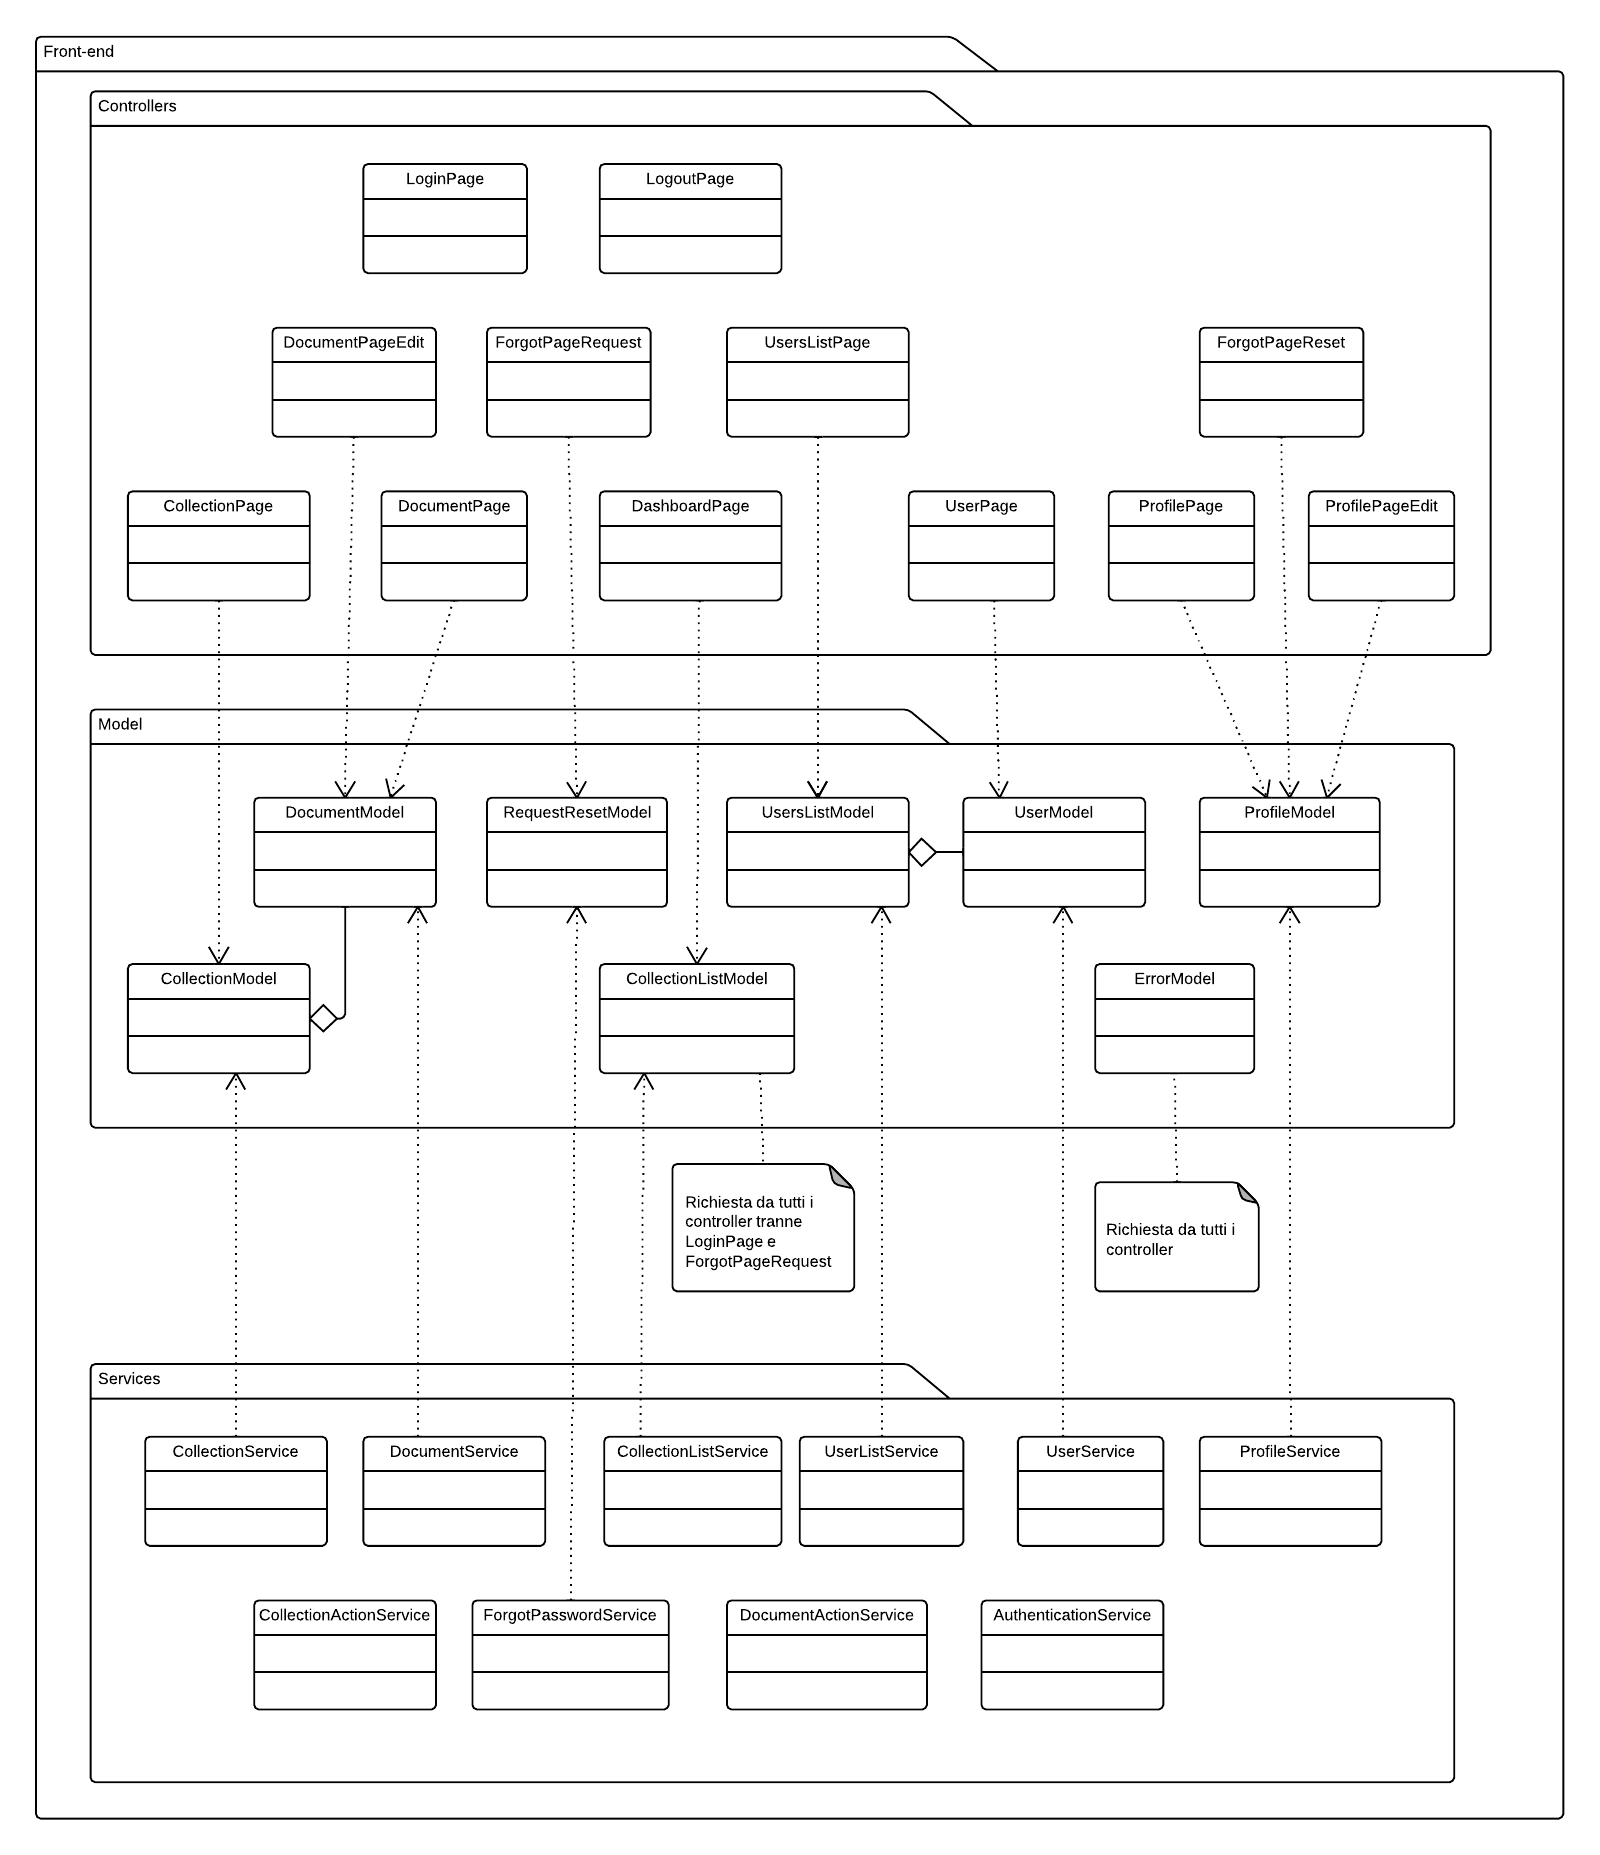
\includegraphics[width=\textwidth]{packages/Front-end.png}  
        \caption{Componente Front-end}
      \end{center}  
    \end{figure} 
  \subparagraph{Descrizione} 
    \begin{itemize}
    \item[] 
    \end{itemize} 
    \subparagraph{Package contenuti} 
    \begin{itemize}
        \item Front-end::Controllers
        \item Front-end::Services
        \item Front-end::Model
    \end{itemize}
  \subsubsection{Front-end::Controllers}
  \paragraph{Informazioni sul package}
    \begin{figure}[H] 
      \begin{center} 
        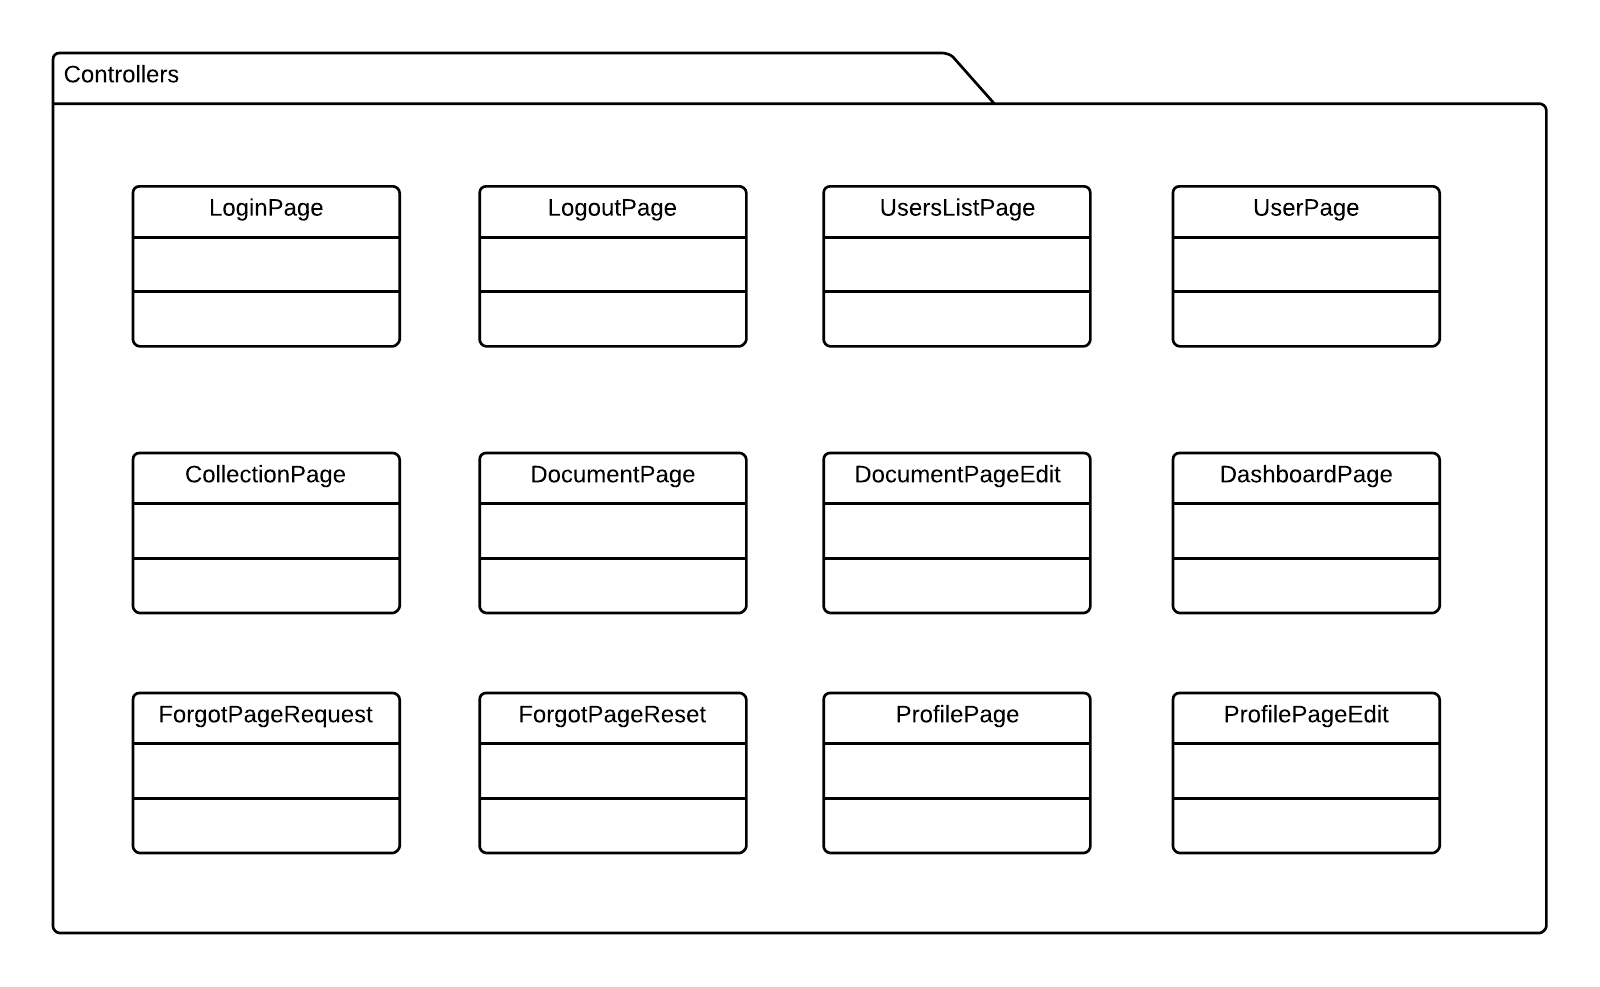
\includegraphics[width=\textwidth]{packages/Front-end::Controllers.png}  
        \caption{Componente Front-end::Controllers}
      \end{center}  
    \end{figure} 
  \subparagraph{Descrizione} 
    \begin{itemize}
    \item[] 
    \end{itemize} 
    \paragraph{Classi}
      \subparagraph{Front-end::Controllers::LoginPage}
        
        \textbf{\\ \\ Descrizione} 
          \begin{itemize}
            \item[] 
          \end{itemize}      
        \textbf{Utilizzo}  
          \begin{itemize}
            \item[] 
          \end{itemize}
      \subparagraph{Front-end::Controllers::LogoutPage}
        
        \textbf{\\ \\ Descrizione} 
          \begin{itemize}
            \item[] 
          \end{itemize}      
        \textbf{Utilizzo}  
          \begin{itemize}
            \item[] 
          \end{itemize}
      \subparagraph{Front-end::Controllers::ForgotPageRequest}
        
        \textbf{\\ \\ Descrizione} 
          \begin{itemize}
            \item[] 
          \end{itemize}      
        \textbf{Utilizzo}  
          \begin{itemize}
            \item[] 
          \end{itemize}
      \subparagraph{Front-end::Controllers::ForgotPageReset}
        
        \textbf{\\ \\ Descrizione} 
          \begin{itemize}
            \item[] 
          \end{itemize}      
        \textbf{Utilizzo}  
          \begin{itemize}
            \item[] 
          \end{itemize}
      \subparagraph{Front-end::Controllers::IndexPage}
        
        \textbf{\\ \\ Descrizione} 
          \begin{itemize}
            \item[] 
          \end{itemize}      
        \textbf{Utilizzo}  
          \begin{itemize}
            \item[] 
          \end{itemize}
      \subparagraph{Front-end::Controllers::UsersIndex}
        
        \textbf{\\ \\ Descrizione} 
          \begin{itemize}
            \item[] 
          \end{itemize}      
        \textbf{Utilizzo}  
          \begin{itemize}
            \item[] 
          \end{itemize}
      \subparagraph{Front-end::Controllers::ShowPage}
        
        \textbf{\\ \\ Descrizione} 
          \begin{itemize}
            \item[] 
          \end{itemize}      
        \textbf{Utilizzo}  
          \begin{itemize}
            \item[] 
          \end{itemize}
      \subparagraph{Front-end::Controllers::DashboardPage}
        
        \textbf{\\ \\ Descrizione} 
          \begin{itemize}
            \item[] 
          \end{itemize}      
        \textbf{Utilizzo}  
          \begin{itemize}
            \item[] 
          \end{itemize}
      \subparagraph{Front-end::Controllers::ShowPageEdit}
        
        \textbf{\\ \\ Descrizione} 
          \begin{itemize}
            \item[] 
          \end{itemize}      
        \textbf{Utilizzo}  
          \begin{itemize}
            \item[] 
          \end{itemize}
      \subparagraph{Front-end::Controllers::ProfilePage}
        
        \textbf{\\ \\ Descrizione} 
          \begin{itemize}
            \item[] 
          \end{itemize}      
        \textbf{Utilizzo}  
          \begin{itemize}
            \item[] 
          \end{itemize}
      \subparagraph{Front-end::Controllers::ProfilePageEdit}
        
        \textbf{\\ \\ Descrizione} 
          \begin{itemize}
            \item[] 
          \end{itemize}      
        \textbf{Utilizzo}  
          \begin{itemize}
            \item[] 
          \end{itemize}
  \subsubsection{Front-end::Services}
  \paragraph{Informazioni sul package}
    \begin{figure}[H] 
      \begin{center} 
        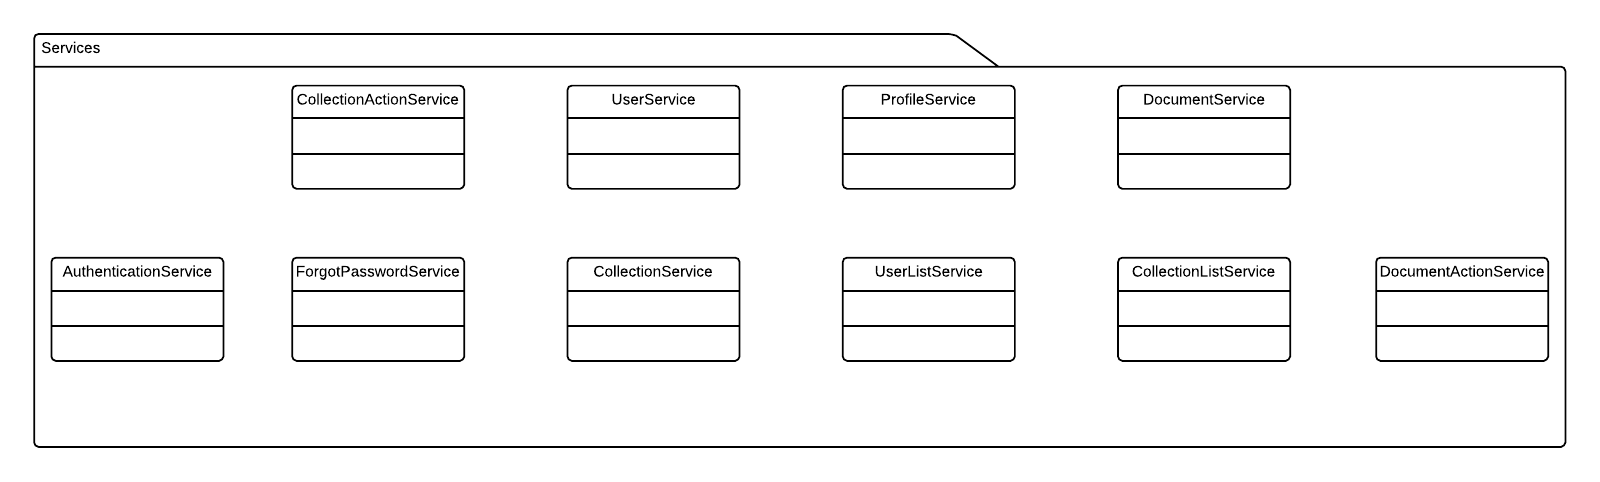
\includegraphics[width=\textwidth]{packages/Front-end::Services.png}  
        \caption{Componente Front-end::Services}
      \end{center}  
    \end{figure} 
  \subparagraph{Descrizione} 
    \begin{itemize}
    \item[] 
    \end{itemize} 
    \paragraph{Classi}
      \subparagraph{Front-end::Services::UserService}
        
        \textbf{\\ \\ Descrizione} 
          \begin{itemize}
            \item[] Questa classe permette il recupero della risorsa REST rappresentante l'utente tramite la chiamata /users/$\{$user_id$\}$
          \end{itemize}      
        \textbf{Utilizzo}  
          \begin{itemize}
            \item[] Le funzionalità offerte dalla classe sono: 
\begin{itemize} 
\item elenco dei dati relativi all'utente. 
\item modifica della password relativa al utente.
\item elevare o declassare un utente ad admin 
\item rimozione dell'utente. 
Tali funzionalità richiedono che l'utente sia un admin.
          \end{itemize}
      \subparagraph{Front-end::Services::AuthenticationService}
        
        \textbf{\\ \\ Descrizione} 
          \begin{itemize}
            \item[] Questa classe permette la creazione e l'eliminazione della sessione utente attraverso le corrispettive chiamate /login e /logout
          \end{itemize}      
        \textbf{Utilizzo}  
          \begin{itemize}
            \item[] La funzionalità offerta dalla classe è quella di poter fornire al Controller lo stato della sessione utente.
          \end{itemize}
      \subparagraph{Front-end::Services::ProfileService}
        
        \textbf{\\ \\ Descrizione} 
          \begin{itemize}
            \item[] Questa classe permette il recupero delle risorsa REST rappresentante il profilo utente tramite la chiamata /profile
          \end{itemize}      
        \textbf{Utilizzo}  
          \begin{itemize}
            \item[] Le funzionalità offerte dalla classe sono:
\begin{itemize}
\item elenco dei dati relativi all'utente
\item modifica dei dati utente
\end{itemize}

Tali funzionalità richiedono che l'utente sia autenticato al sistema.
          \end{itemize}
      \subparagraph{Front-end::Services::UserListService}
        
        \textbf{\\ \\ Descrizione} 
          \begin{itemize}
            \item[] Questa classe permette il recupero delle risorse REST rappresentanti gli utenti registrati all'applicazione tramite la chiamata /users
          \end{itemize}      
        \textbf{Utilizzo}  
          \begin{itemize}
            \item[] La funzionalità offerta dalla classe è quella di poter fornire al Controller la lista degli utenti presenti nel database delle credenziali.
Tale funzionalità richiede che l'utente sia un admin.
          \end{itemize}
      \subparagraph{Front-end::Services::CollectionListService}
        
        \textbf{\\ \\ Descrizione} 
          \begin{itemize}
            \item[] Questa classe permette il recupero delle risorse REST rappresentanti le Collections tramite la chiamata /collections
          \end{itemize}      
        \textbf{Utilizzo}  
          \begin{itemize}
            \item[] La funzionalità offerta dalla classe è quella di poter fornire al Controller la lista delle Collections registrate dallo sviluppatore e presenti nel database delle collections.
Tale funzionalità richiede che l'utente sia registrato.
          \end{itemize}
      \subparagraph{Front-end::Services::CollectionActionService}
        
        \textbf{\\ \\ Descrizione} 
          \begin{itemize}
            \item[] Questa classe permette l'esecuzione (nel backend) delle azioni personalizzate di una Collection tramite la chiamata /action/$\{$action name$\}$/$\{$collection name$\}$
          \end{itemize}      
        \textbf{Utilizzo}  
          \begin{itemize}
            \item[] La funzionalità offerta dalla classe è quella di poter fornire al Controller il risultato dell'azione personalizzata definita dallo sviluppatore su una Collection.
          \end{itemize}
      \subparagraph{Front-end::Services::DocumentActionService}
        
        \textbf{\\ \\ Descrizione} 
          \begin{itemize}
            \item[] Questa classe permette l'esecuzione (nel backend) delle azioni personalizzate di un Document tramite la chiamata /action/$\{$action name$\}$/$\{$collection name$\}$/$\{$document id$\}$
          \end{itemize}      
        \textbf{Utilizzo}  
          \begin{itemize}
            \item[] La funzionalità offerta dalla classe è quella di poter fornire al Controller il risultato dell'azione personalizzata definita dallo sviluppatore su un Document.
          \end{itemize}
      \subparagraph{Front-end::Services::CollectionService}
        
        \textbf{\\ \\ Descrizione} 
          \begin{itemize}
            \item[] Questa classe permette il recupero della risorsa REST rappresentante la Collection tramite la chiamata  /collection/$\{$collection_name$\}$
          \end{itemize}      
        \textbf{Utilizzo}  
          \begin{itemize}
            \item[] La funzionalità offerta dalla classe è quella di poter fornire al Controller la lista di Document presenti nella Collection.
          \end{itemize}
      \subparagraph{Front-end::Services::ForgotPasswordService}
        
        \textbf{\\ \\ Descrizione} 
          \begin{itemize}
            \item[] Questa classe si occupa di inviare al server una richiesta di recupero password tramite la chiamata /password/lost e la conseguente modifica attraverso la chiamata /password/reset.
          \end{itemize}      
        \textbf{Utilizzo}  
          \begin{itemize}
            \item[] La funzionalità offerta dalla classe è quella di interagire col server delegando quest'ultimo all'invio di una mail all'utente per il recupero della password e successivamente alla sua modifica.
          \end{itemize}
      \subparagraph{Front-end::Services::DocumentService}
        
        \textbf{\\ \\ Descrizione} 
          \begin{itemize}
            \item[] Questa classe permette il recupero delle risorse REST rappresentanti i Document di una Collection tramite la chiamata /collections/$\{$collection_name$\}$/$\{$document id$\}$
          \end{itemize}      
        \textbf{Utilizzo}  
          \begin{itemize}
            \item[] Le funzionalità offerte dalla classe sono: 
\begin{itemize} 
\item elenco dei dati relativi al Document 
\item modifica dei dati relativi al Document
\item rimozione del Document 
\end{itemize} 
Tali funzionalità richiedono che l'utente sia autenticato al sistema.
          \end{itemize}
  \subsubsection{Front-end::Model}
  \paragraph{Informazioni sul package}
    \begin{figure}[H] 
      \begin{center} 
        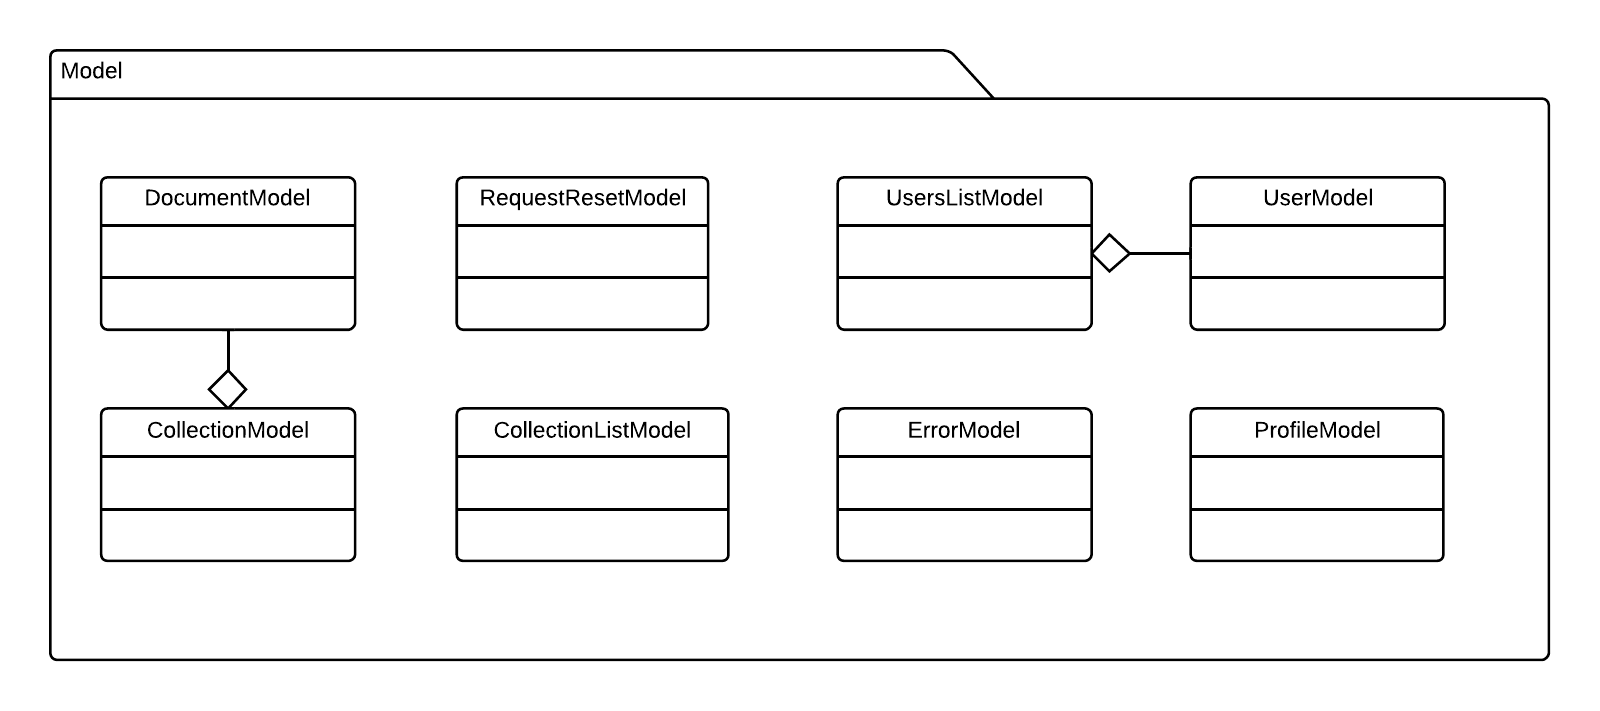
\includegraphics[width=\textwidth]{packages/Front-end::Model.png}  
        \caption{Componente Front-end::Model}
      \end{center}  
    \end{figure} 
  \subparagraph{Descrizione} 
    \begin{itemize}
    \item[] 
    \end{itemize} 
    \paragraph{Classi}
      \subparagraph{Front-end::Model::UserModel}
        
        \textbf{\\ \\ Descrizione} 
          \begin{itemize}
            \item[] 
          \end{itemize}      
        \textbf{Utilizzo}  
          \begin{itemize}
            \item[] 
          \end{itemize}
      \subparagraph{Front-end::Model::UserListModel}
        
        \textbf{\\ \\ Descrizione} 
          \begin{itemize}
            \item[] 
          \end{itemize}      
        \textbf{Utilizzo}  
          \begin{itemize}
            \item[] 
          \end{itemize}
      \subparagraph{Front-end::Model::ResetModel}
        
        \textbf{\\ \\ Descrizione} 
          \begin{itemize}
            \item[] 
          \end{itemize}      
        \textbf{Utilizzo}  
          \begin{itemize}
            \item[] 
          \end{itemize}
      \subparagraph{Front-end::Model::IndexModel}
        
        \textbf{\\ \\ Descrizione} 
          \begin{itemize}
            \item[] 
          \end{itemize}      
        \textbf{Utilizzo}  
          \begin{itemize}
            \item[] 
          \end{itemize}
      \subparagraph{Front-end::Model::ShowModel}
        
        \textbf{\\ \\ Descrizione} 
          \begin{itemize}
            \item[] 
          \end{itemize}      
        \textbf{Utilizzo}  
          \begin{itemize}
            \item[] 
          \end{itemize}
      \subparagraph{Front-end::Model::ErrorModel}
        
        \textbf{\\ \\ Descrizione} 
          \begin{itemize}
            \item[] 
          \end{itemize}      
        \textbf{Utilizzo}  
          \begin{itemize}
            \item[] 
          \end{itemize}
      \subparagraph{Front-end::Model::ProfileModel}
        
        \textbf{\\ \\ Descrizione} 
          \begin{itemize}
            \item[] 
          \end{itemize}      
        \textbf{Utilizzo}  
          \begin{itemize}
            \item[] 
          \end{itemize}